% Chapter 4

\chapter{Findings} % Main chapter title

\label{Chapter4} % For referencing the chapter elsewhere, use \ref{Chapter1} 

This Chapter presents the results of the tests discussed in \ref{Chapter3}. Also included is a discussion of applications that were successfully run over the network. Finally, an analysis of the results, and a discussion of error is presented. 

%----------------------------------------------------------------------------------------

% Define some commands to keep the formatting separated from the content 
%\newcommand{\keyword}[1]{\textbf{#1}}
%\newcommand{\tabhead}[1]{\textbf{#1}}
%\newcommand{\code}[1]{\texttt{#1}}
%\newcommand{\file}[1]{\texttt{\bfseries#1}}
%\newcommand{\option}[1]{\texttt{\itshape#1}}

%----------------------------------------------------------------------------------------

\section{Results}

\subsection{Network Benchmarks}

\begin{figure}
	\centering
	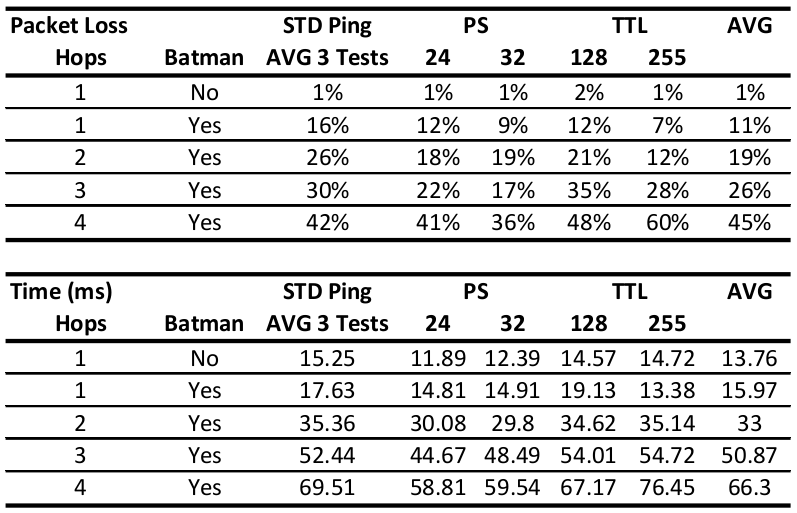
\includegraphics[scale=0.5]{902sheet}
	\caption{The data received from operating at 902/915 MHz.}
	\label{fig:902}
\end{figure}

\begin{figure}
	\centering
	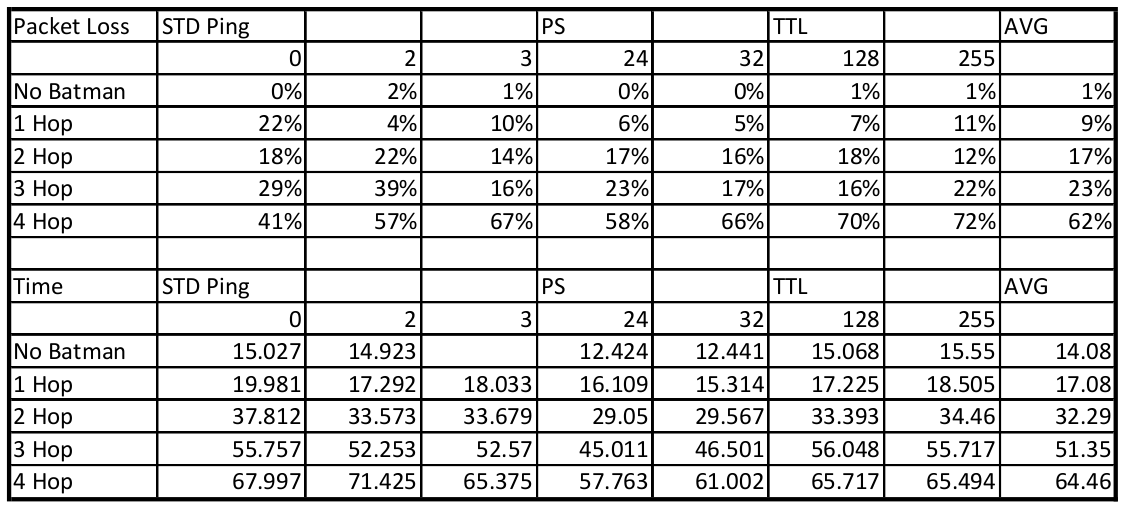
\includegraphics[scale=0.5]{2400}
	\caption{The data received from operating at 2.4/2.5 GHz.}
	\label{fig:2400}
\end{figure}

\begin{figure}
	\centering
	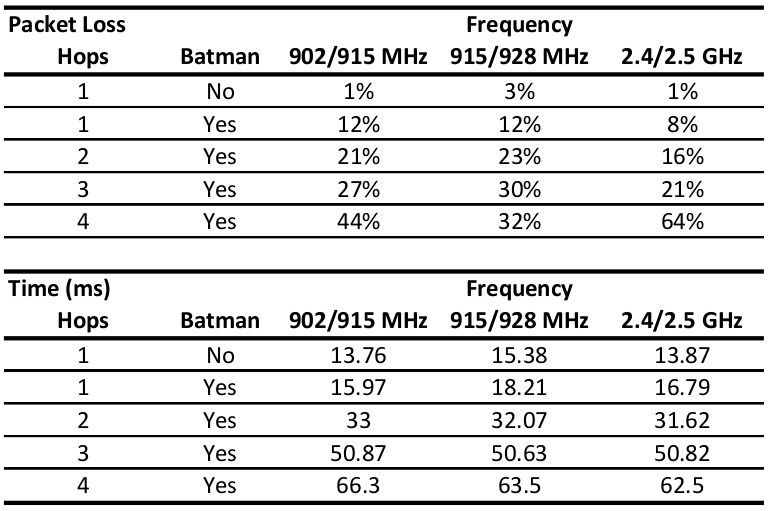
\includegraphics[scale=0.5]{alldata}
	\caption{The Averages from all three tests.}
	\label{fig:alldata}
\end{figure}

The results of the Network Benchmark tests from section 4 part A are summarized in Figure \ref{fig:alldata}. In all cases, the single point to point communication, without the batman-adv protocol running, resulted in a much lower packet loss. This served as our control group. However, in the two sets of lower frequency ratings, the packet loss remained below 50\%. Also, the increase in time as hops were added has a roughly linear change. This indicates the overhead of adding more hops is not unmanageable. A full listing of tests run for the 902/915 MHz, and 2.4/2.5 GHz cases are provided in Figure \ref{fig:902} and Figure \ref{fig:2400} respectively. These tables show that running at the higher frequencies causes the SDRN to drop a lot more packets, especially when moving through the full four hops.  


\subsection{Route Changes}

\begin{figure}
	\centering
	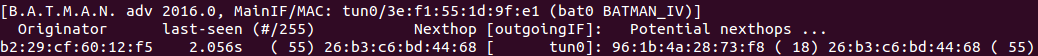
\includegraphics[scale=0.4]{2PotentialHops}
	\caption{The initial condition from the test presented in Section 4 B, where there are two possible routes the packet can take. The output is from running batctl. The link quality is listed under the column labeld (\#/255). A higher number represents a better quality connection.}
	\label{fig:2Hops}
\end{figure}

\begin{figure}
	\centering
	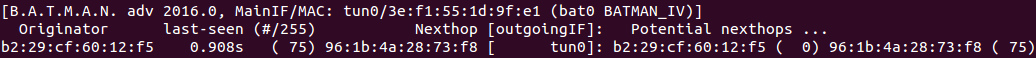
\includegraphics[scale=0.4]{hopchange}
	\caption{After the gain is reduced in the test presented in Section 4 B, the packets are now routing through a different node.}
	\label{fig:NewHop}
\end{figure}

The route changing feature of batman-adv showed success with our test setup from section 4 part B. Initially, batctl reported two possible links, one with a link quality of 55, and the other with a link quality of 18. As we decreased the gain of the intermediate node, the link quality reported by batctl also decreased. Eventually, batman-adv switched and began using the other node. At this point, it no longer saw the original node, and reported a link quality of 75 on the alternate one. The initial setup can be seen in Figure \ref{fig:2Hops}. After the change, the routing table appeared as it does in Figure \ref{fig:NewHop}. This feature works in the SDR system, and can continue to be used without significant changes.  

\subsection{Frequency Changes}

\begin{figure}
	\centering
	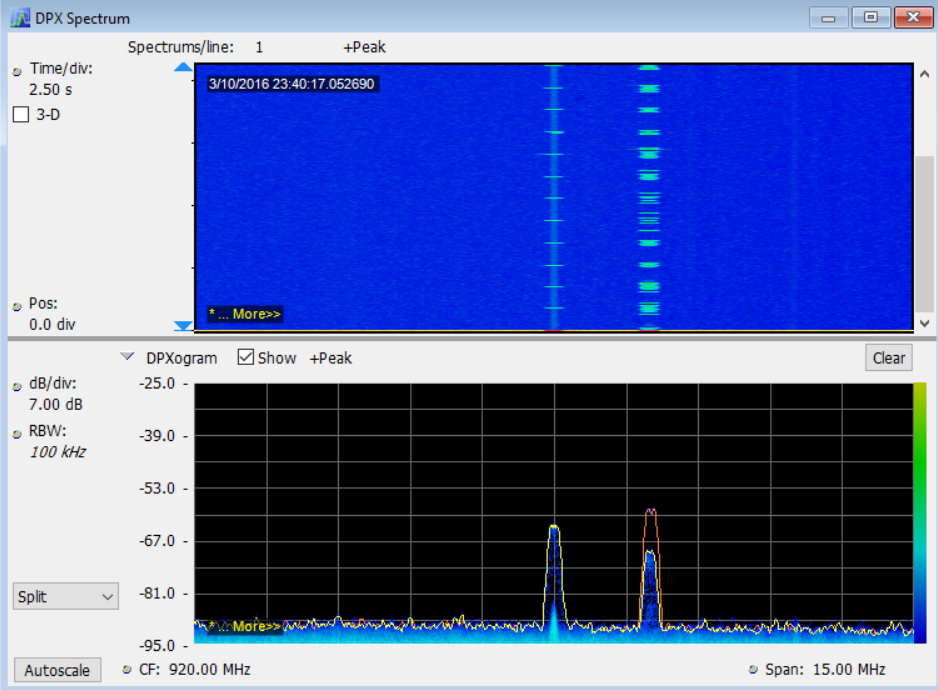
\includegraphics[scale=0.4]{FrequencyShift922-920}
	\caption{The result of using ALFRED to shift frequencies. One node is left behind as the others move to the new channel. Image collected using the Tektronix RSA306 Spectrum Analyzer}
	\label{fig:freqshift}
\end{figure}


Using A.L.F.R.E.D. to distribute frequency hopping showed mixed results. Using the setup from section 4 part C, we were able to get the nodes to change frequency in unison, but not reliably. A.L.F.R.E.D. itself is designed for a traditional Wi-Fi environment, and therefore does not have an expectation that the other nodes will become completely unreachable due to changes in operating frequency \cite{0015}. We were finding that some nodes would switch before A.L.F.R.E.D. had propagated the data table to the other nodes. This would leave one node with an out-of-date table, meaning it would not make the frequency change. In the current iteration of the project, there is no way for these orphaned nodes to find the rest of the network again. Figure \ref{fig:freqshift} shows a situation in which four out of five nodes were able to make the jump, with one node remaining at the original frequency.

\section{Applications}

%% Change the below if more tests are able to be run, there is probably some good quantitiative data that can be captured from SCP at least

Several application level programs were run over the network. Each application was run in both a single and multihop setting. Qualitative measurements were recorded as it was difficult to make quanititve measurements about the effectiveness of the network. The first test was run using Secure Shell (SSH). On one computer, a user would use ssh to connect to a remote computer and run a few commands to confirm operation. Next, Secure Copy (SCP) was used to transmit a file from one computer to another. A simple chat application was built in both Python and Erlang to demonstrate the ability to communicate over the network. 


%----------------------------------------------------------------------------------------

\section{Data Analysis}

In an ideal situation, we would see minimal packet loss despite introducing batman-adv and multihopping into the network. Additional tests will need to be run to discover what causes the 1 hop with batman-adv to drop many more packets than 1 hop without batman-adv. It is possible the packets are dropped as routing table information is shared, but this has not been confirmed yet. 

It is important to notice that packet loss and round trip time of packets increases lineraly with each hop. This is good, as it indicates each hop adds a finite amount of delay and packet loss. It would be unlikely that the delay would be constant when adding more hops, so a linear time increase is good. 

Another interesting issue with this test was that we had to stagger the operating frequencies to force the straight line topology we were looking for. Batman-adv worked very well at finding alternative paths to each node in the network. However, if the tests were left running for long periods of time it was possible the network would have been able to reconfigure into a topology other than a straight line chain. Therefore, it was necessary to manually ensure that the network would stay in the desired configuration in order to maintain a valid test. 

The route changing feature of batman-adv worked fine with the SDR hardware. Initially, there was uncertantity if batman-adv would be able to compute a proper metric for the link quality of each node. This link quality metric is what batman-adv uses to determine the best ``next hop'' to reach a different node. However, our tests showed the routing table could be properly built and updated as link quality decreased.

Our tests on A.L.F.R.E.D. showed that it was possible to exchange frequency information over the network. However, the tests revealed that this was a very unreliable method. There is no way to ensure that A.L.F.R.E.D. had shared changes to its data table to all other nodes on the network. This meant that some nodes would change their frequency while others would remain at the older frequency. In some CRAHNs, the nodes act as secondary users and transmit on a channel when it is unoccupied. If this was being used to avoid a primary user, a long delay would not be acceptable as it would interfere with the PU's use of the spectrum. Therefore, a new implementation of this feature will need to be produced. 



%----------------------------------------------------------------------------------------

\section{Assumptions and Discussion of Error}

One assumption is that the straight line configuration shown in Figure \ref{fig:HopMess} reflects how the network would behave in a full scale environment. Here we are using this configuration to determine the overhead associated with each additional hop. However, in a more robust network configuration it is likely there will be more than one path to any given node. These additional paths may be necessary to lower the overall packet loss of the network. It may be more appropriate to test this type of configuration in simulation rather than in the real world. 

We also did not test these setups in an anechoic chamber. Therefore, it is not possible to know how reflections influenced our data set. Reflections of RF waveforms can cause both constructive and destructive interference. This indicates that the reflections could alter the signal quality at any given node.  

The experiments were performed over a 24 hour period. Therefore, some tests were performed while the lab was actively being used by other researchers and some were performed while the room was empty. This again could have impacted the results. The reflectivity of the room is altered with people present. Also, the overall level of RF noise will be higher with people present as they will likely be using cell phones and computers with wireless capabilities. 

A uniform operating pattern in each node and in each antenna is assumed. Without the necessary equipment, it is impossible to truly characterize the antennas or transmission patterns of the SDRs. This is not likely to be a source of error based upon the information in the data sheets, but it is something to be aware of. 


%----------------------------------------------------------------------------------------

%\section{Error Bars}

%----------------------------------------------------------------------------------------

